%%%%%%%
% Ch2 %
%%%%%%%

\chapter{Diode rectifiers}
	
	Diode rectifiers are simple and cheap and they don't need any adjustment prior to their employment. They provide a DC voltage primarily constant from an AC voltage. There are two kinds of load to supply: those who need a smooth DC voltage and those who need a limited voltage distortion. Electronic devices belong to the first category, that's why we find capacitors connected between the output terminals. Those capacitors will smooth the rectified signal. DC machines and RLE loads belong to the second category. They need thyristor rectifiers (\textbf{controllable}) because the diode rectifier is uncontrollable.
	The list of symbols needed in this chapter is just below.
	
	\begin{center}
	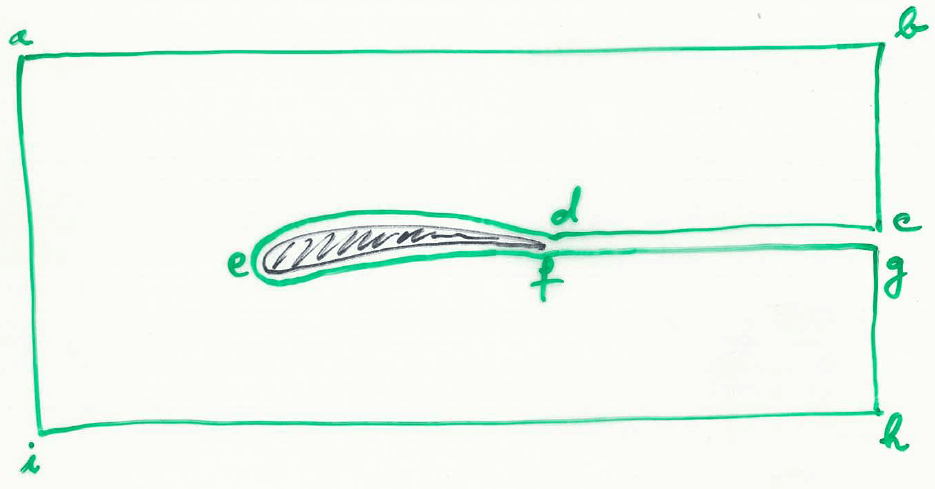
\includegraphics[scale=0.45]{ch2/1}
	\captionof{table}{List of symbols.}
	\end{center}
	\newpage
	
	\section{Characteristics of diodes}
		This figure shows the symbol of a diode as well as three characteristics depending on the accuracy needed. The diode \textbf{conducts} if $v_D=v_{AK}$ (\textbf{threshold voltage}). Voltage will therefore barely depend on current $i_D$.
		
		\begin{center}
		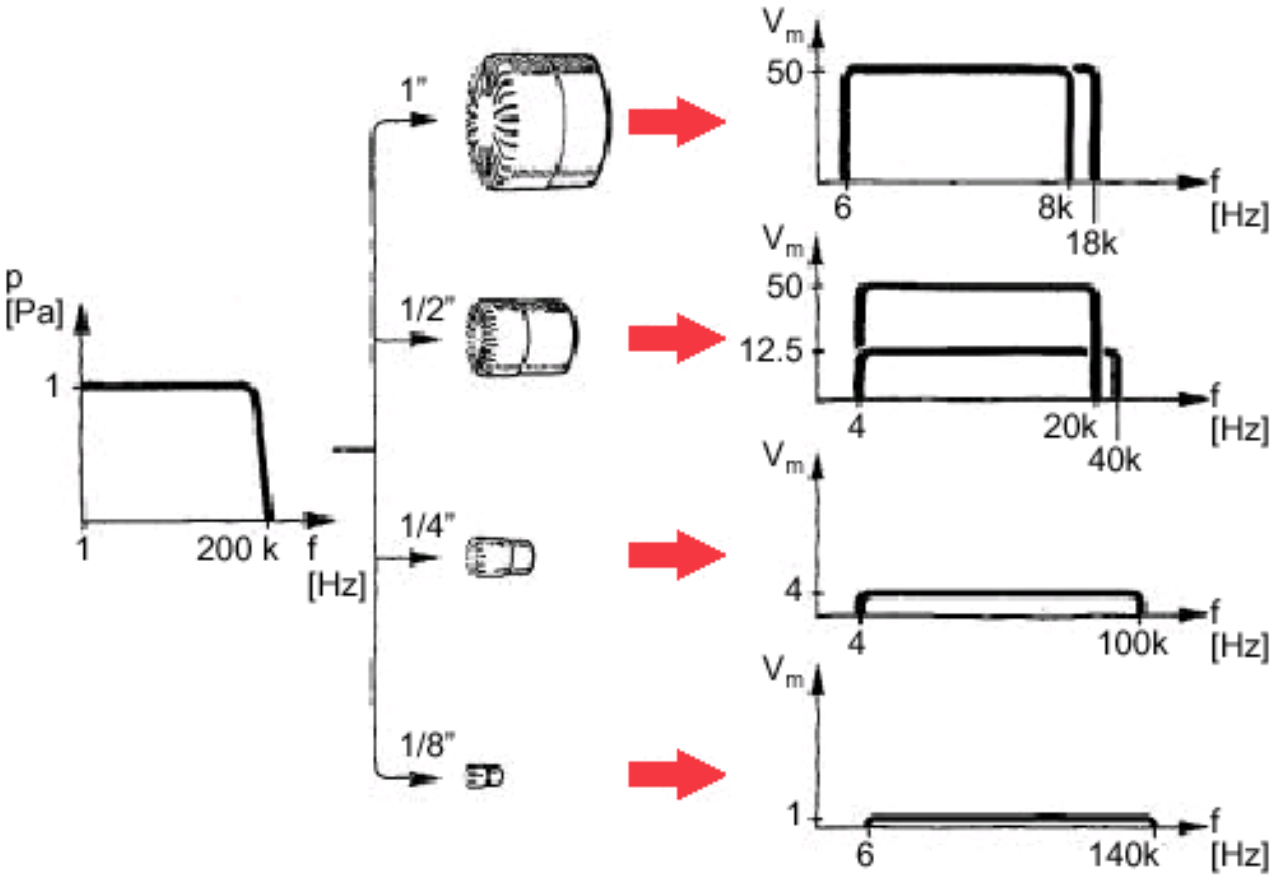
\includegraphics[scale=0.45]{ch2/2}
		\captionof{figure}{}
		\end{center}			
		
		The maximum current admitted by a diode (during long intervals of time) represented by $I_{D,max}$ in the figure depends on its construction, its size and its cooling system and it can reach up to some kA.
		Heat transfer to the radiator is essential in the conception and employment of power electronics diodes. As other semi-conducting components, diodes have little thermal inertia because of their size. Its temperature can therefore rise very fast.
		According to the simplified characteristic, conduction losses are approximated as follows:
		
		\begin{equation}
			v_D = V_{D,on} + R_{D,on} i_D
		\end{equation}
		where $V_{D,on}$ is the \textbf{threshold voltage} and is approximately $1V$. Besides low voltage applications (less than 10 volts), we will neglect this voltage $v_D$ because it has little influence on the characteristics of diode integrated converters. However, we will not forget the fact that the voltage drop corresponds to the instantaneous conduction losses $P_D(t) = v_D(t)i_D(t)$ and the evacuation of these losses is essential. \\
	
        In power electronics, diodes are used at low commutation frequencies ($50 - 60 Hz$).
	
	\section{Inductive load and elementary rectifiers}
		\subsection{Elementary rectifier circuits, generic RLE load}
		In order to study some elementary circuits employing one or two diodes and other circuits such as diode bridges, we will consider a generic RLE load. R, L and E are constant, which means that their variation over a fundamental period of the AC source is arbitrarily small. Such a load might represent, for example, the induced circuit of a DC machine ($E_{dc} \neq 0$) or its excitation circuit ($E_{dc}=0$). The differential equation of the voltage over the load is:
		\begin{equation}
			v_{dc} = E_{dc} + R_{dc}i_{dc} + L_{dc}\frac{di_{dc}}{dt}.
		\end{equation}
			
		At steady state and by introducing the \textbf{average voltage} $V_{dc}$ and the \textbf{average current} $I_{dc}$, we get:
			
			\begin{equation}
				V_{dc} = E_{dc} + R_{dc} I_{dc}.
			\end{equation}
			
			The load is fed by a diode rectifier, thus $i_{dc}$ and $I_{dc}$ cannot be negative and if $E_{dc}\geq v_{ac}$ then the current stops flowing. We can therefore write:
			\begin{equation}
				I_{dc} = max\left(\frac{V_{dc} - E_{dc}}{R_{dc}}, 0\right).
			\end{equation}
			The inductance of the load will smooth the current. This effect will be greater as the time constant $\tau = L_{dc}/R_{dc}$ becomes greater with respect to the period $T=1/f$ of the grid. For single-phase bridges and three-phase bridges the period concerning us will be $T/2$ and $T/6$ respectively. In the case of an MCC, the fluctuations of the voltage imposes a fluctuation of the current and, therefore, a fluctuation of the \textbf{electromagnetic torque}, which is troubling. Thus, we can add an outer inductance if the inner one is not enough, at the expenses of losing dynamic performance. 

		\subsection{Elementary rectifier circuit with an RE load}
			\subsubsection{With an R load}
			    We will begin by analyzing the simpler case, the one of an R load. The figure hereafter represents a circuit with an AC ideal voltage source of frequency $f$ linked to an ideal diode and a resistance $R_{dc}$. In this case, $i_{ac}(t)=i_{dc}(t)$. The diode isn't in direct bias unless $v_{ac}(t)>0$. When that happens we have $v_{dc}(t)=v_{ac}(t)$ and $i_{dc}=v_{ac}(t)/R_{dc}$. The diode will stop the current when $v_D=v_{ac}<0$, and we will have $v_{dc}=0=i_{dc}$.
				
				\begin{center}
					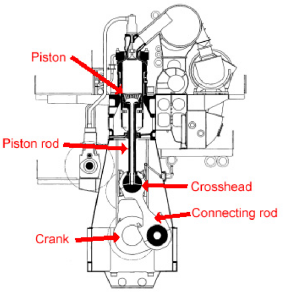
\includegraphics[scale=0.45]{ch2/3}
					\captionof{figure}{}
				\end{center}
				
				We obtain the average value of the voltage by integrating the instantaneous voltage over half a conduction period:
				\begin{equation}
					V_{dc} = \frac{1}{2\pi} \int _0^\pi \sqrt{2}V_{ac}\sin (\omega t) \, d\omega t = \underbrace{\frac{\sqrt{2}}{\pi}}_{0.450} V_{ac}.
					\label{eq:2.5}
				\end{equation}
				
				The rectified voltage and its respective current $i_{dc}=i_{ac}$ are highly distorted, all the harmonics of frequency $kf$ are present (we don't have half-wave symmetry). This circuit is not very appropriate for practical cases. In addition, having a DC current come from an AC source will generate problems. 
				
			\subsubsection{With an RE load}
			
			    Now we have a DC voltage source added to the load. It might be the case of a battery and its inner resistance. 
				
				\begin{center}
				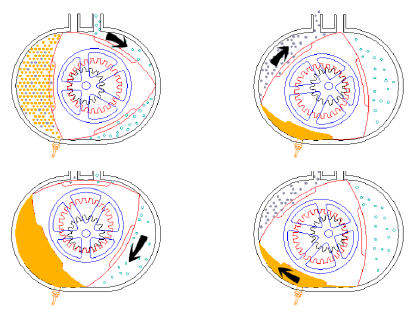
\includegraphics[scale=0.45]{ch2/4}
				\captionof{figure}{}
				\end{center}	
				
				When the diode conducts we have: $v_{ac}(t) = v_{dc}(t) = E_{dc} + R_{dc}I_{dc}$. This happens if the condition $(v_{ac}-E_{dc})/R_{dc}>0$ (that is to say $v_{ac}>E_{dc}$) is respected. When the diode blocks the passage of the current we have $v_{dc} = E_{dc}$. The DC quantities are distorted and every harmonic of frequency $kf$ will appear in the spectre.
				The conduction intervals will have an extension $T_c$ where $\theta _c = \omega T_c$. Its duration can be calculated as follows:
				\begin{equation}
					E_{dc} = \hat{V}_{ac} \sin \left(\frac{\pi}{2} - \frac{\theta _c}{2}\right) = \hat{V}_{ac} \cos \frac{\theta _c}{2} \qquad \Rightarrow \qquad \theta _c = 2 \arccos \frac{E_{dc}}{\hat{V}_{ac}}
				\end{equation}
				In this equation we can ascertain that as $E_{dc}$ grows closer to $\hat{V}_{ac}$ the extension of the intervals decreases. The average voltage $V_{dc}$ can be obtained by integrating over a conduction interval $\theta _c$ and the remaining $2\pi - \theta _c$ : 
				\begin{equation}
				\begin{aligned}
					\frac{V_{dc}}{\hat{V}_{ac}} &= \frac{1}{2\pi\hat{V}_{ac}} \left[ \int _0 ^{2 \arccos \frac{E_{dc}}{\hat{V}_{ac}}} \hat{V}_{ac} \sin \omega t\,  d\omega t + \int _{2 \arccos \frac{E_{dc}}{\hat{V}_{ac}}} ^{2\pi} E_{dc} \, d\omega t \right]\\
								&= \frac{1}{\pi} \sqrt{1 - \left(\frac{E_{dc}}{\hat{V}_{ac}}\right)^2} + \left(1- \frac{1}{\pi} \arccos \frac{E_{dc}}{\hat{V}_{ac}} \right)
				\end{aligned}
				\end{equation}
				
	\subsection{Elementary rectifier circuit with a free-wheeling diode}
		\begin{wrapfigure}[11]{l}{4.7cm}
		\vspace{-5mm}
		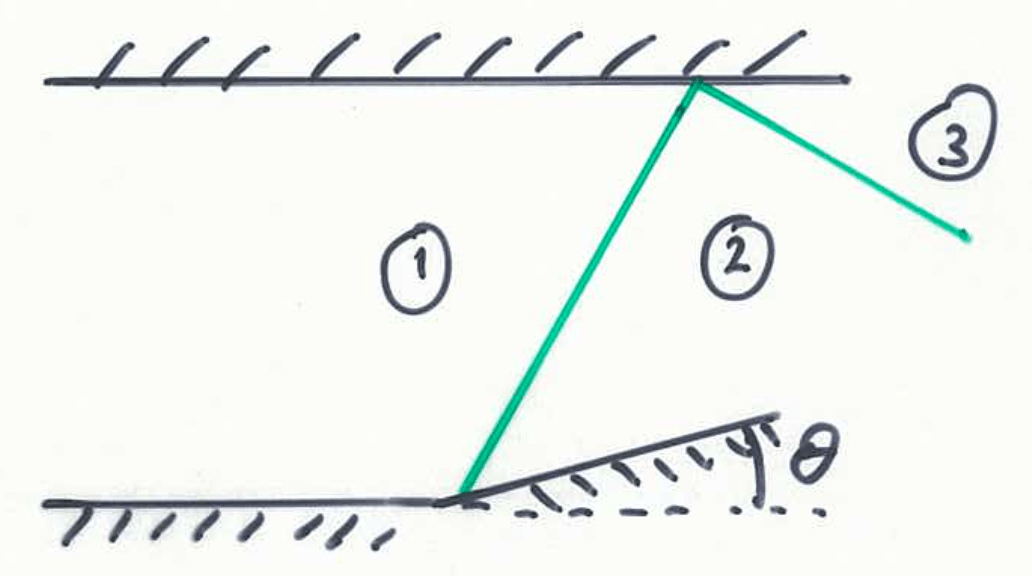
\includegraphics[scale=0.25]{ch2/5}
		\captionof{figure}{}
		\end{wrapfigure}
		In the figure we can observe two diodes D1 and D2, the first one will work the same way as before and the second one (free wheeling-diode) will be an extra path for the current going through the load to follow. The AC load is depicted by its equivalent without a load: a voltage source $v_{ac}^0(t)$ and an inner inductance $L_{ac}$.
		First we will consider the case where $L_{dc} \rightarrow \infty$. Such an inductance will perfectly smooth the current $i_{dc} = I_{dc}$. It remains a single track rectifier because the current is not alternative. 
		
		\ \\
		\subsubsection{Ideal AC voltage source and infinitely inductive load}
		
		    We will begin considering that the AC voltage source is ideal, that is to say $L_{ac} = 0$; and the DC inductance $L_{dc} = \infty$ : 
			\begin{equation}
				i_{dc}(t) = I_{dc} = i_{ac}(t) + i_{D2}(t)
			\end{equation}
			
			We can easily conclude that the load will be fed by the supply during positive alternations and by the free-wheeling diode during negative alternations. The commutation between the diodes is supposed to be instantaneous. The average value of the voltage can therefore be calculated as in \eqref{eq:2.5}. During negative alternations, as D2 lets the current pass, $-v_{D2} = v_{dc} = 0$ and all the voltage appears on D1.  
			
		\subsubsection{Non-ideal AC voltage source and infinitely inductive load}
			\begin{wrapfigure}[10]{l}{5.8cm}
			\vspace{-5mm}
			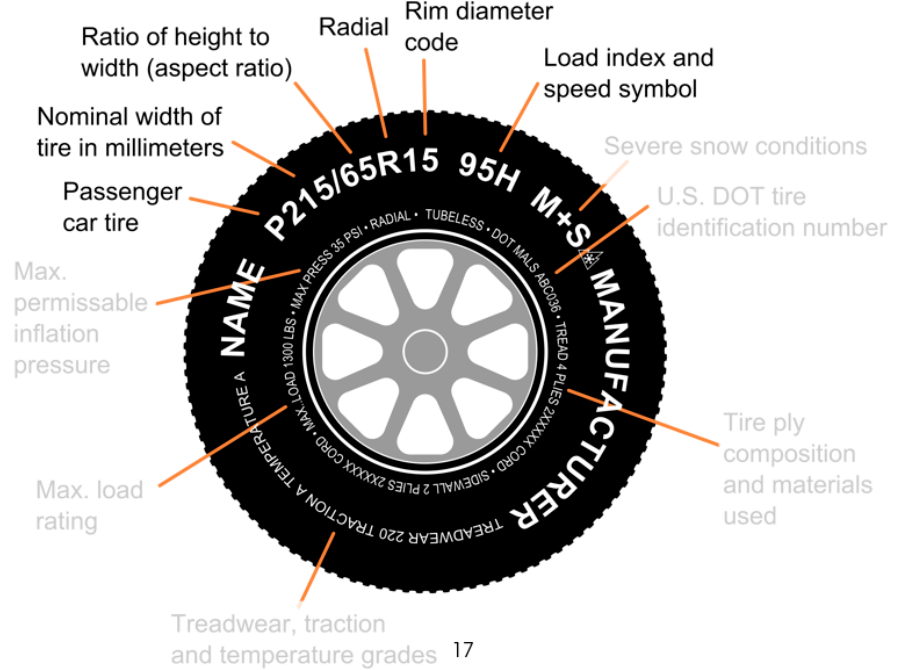
\includegraphics[scale=0.3]{ch2/6}
			\captionof{figure}{}
			\end{wrapfigure}
			Now, $L_{ac}$ prevents instantaneous variations of the current during commutations. The interval, referred to by $T_{com}$, during which both diodes conduct simultaneously can also be called \textbf{encroachment} or \textbf{overlapping} interval. The equation reigning over the commutation between diodes is:
			\begin{equation}
				v_{ac}^0 (t) = \sqrt{2} V_{ac}^0 \sin \omega t = L_{ac}\frac{di_{ac}(t)}{dt}.
				\label{eq:2.9}
			\end{equation}
			During these commutations, the output voltage \\$v_{dc}(t) = - v_{D2}(t) = 0$. In addition, as we consider an infinitely inductive load , the DC current is constant even during commutation intervals. That means: $i_{dc}(t) = I_{dc} = i_{D2}(t) + i_{ac}(t)$.
			If we integrate \eqref{eq:2.9} over a commutation from D2 to D1 as follows: 
			\begin{equation}
			\begin{aligned}
				&\int _0 ^{\omega T_{com}} \sqrt{2} V_{ac}^0 \sin \omega t \, d\omega t = \int _0 ^{I_{dc}} \omega L_{ac}\, di_{ac} \\
				\Leftrightarrow \quad &\sqrt{2} V_{ac}^0 (1- \cos \omega T_{com}) = \omega L_{ac} I_{dc}\\
				\Leftrightarrow \quad &\theta _{com} = \omega T_{com} = \arccos \left( 1 - \frac{\omega L_{ac}}{\sqrt{2} V_{ac}^0}I_{dc} \right)
				\end{aligned}
			\end{equation}
			
			We can ascertain that the higher the current and the inductance are the longer the commutation is. The commutation from $D_1$ to $D_2$ will always take place when $v_{dc} = 0$. The lag of the increase of the voltage will induce a reduction of the average value of the voltage referred to by $\Delta V_{com}$ : 			
			\begin{equation}
				\Delta V_{com} = \frac{1}{2\pi} \int _0 ^{\omega T_{com}} v_{ac}^0(t) \, d\omega t = \frac{1}{2\pi} \int _0 ^{\omega T_{com}} \omega L_{ac}\frac{di_{ac}}{dt} \, dt = \frac{\omega L_{ac}}{2\pi} I_{dc}.
 			\end{equation}
 			
            We reach the same conclusions for the average value of the voltage drop.
 
 		\subsubsection{Thevenin equivalent of the DC side}
 			
			\begin{wrapfigure}[6]{r}{4.2cm}
			\vspace{-5mm}
			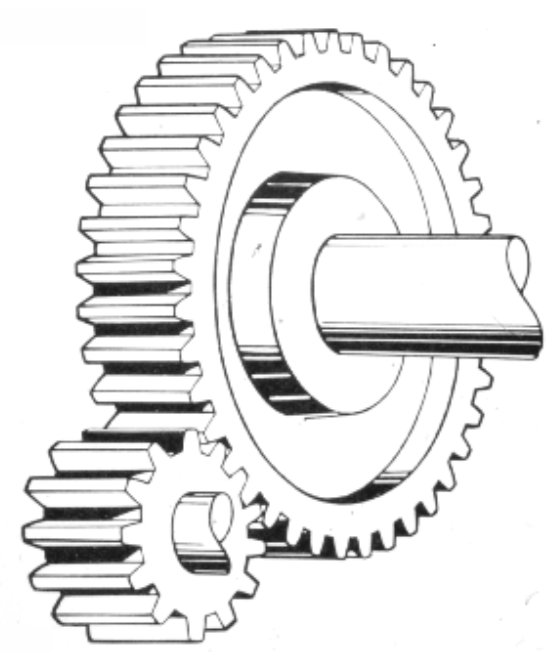
\includegraphics[scale=0.4]{ch2/7}
			\captionof{figure}{}
			\label{fig:2.6}
			\end{wrapfigure} 			
			
			If we take into account the voltage drop in the diodes, we have: 
 			\begin{equation}
 				V_{dc} = \underbrace{0.45 V_{ac} - V_{D,on}}_{V_{dc}^0} - \underbrace{(R_{D,on}+\frac{\omega L_{ac}}{2\pi})}_{R_{i,dc}} I_{dc}
			\end{equation} 	
			where the elements of the equation are gathered to form the Thevenin equivalent of the AC source and both diodes (non-ideal diodes with $V_{dc}^0$ and inner resistance $R_{i,dc}$). In \autoref{fig:2.6}, we can find the duty point. There are no Joule losses associated to $R_{i,dc}$. 
			
		\subsubsection{Non infinitely inductive load}
		
            For a non-ideal case, that is to say a real load and a real inductance $L_{dc}$, we can distinguish two cases. Continuous conduction, which results in an always positive distorted current $i_{dc}$. And the case where the current is discontinuous $i_{dc} = 0$ during some time intervals. When there is  \textbf{continuous conduction}, the equations of $\theta _{com}$ and $\Delta V_{com}$ remain good approximations. However, when we have \textbf{discontinuous conduction}, these equations are not valid and the commutation from $D1$ to $D2$ doesn't exist anymore. 
			
\section{Single-phase and three-phase bridges - basic formulas for the average output voltage}
	\begin{wrapfigure}[7]{l}{7.5cm}
	\vspace{-5mm}
	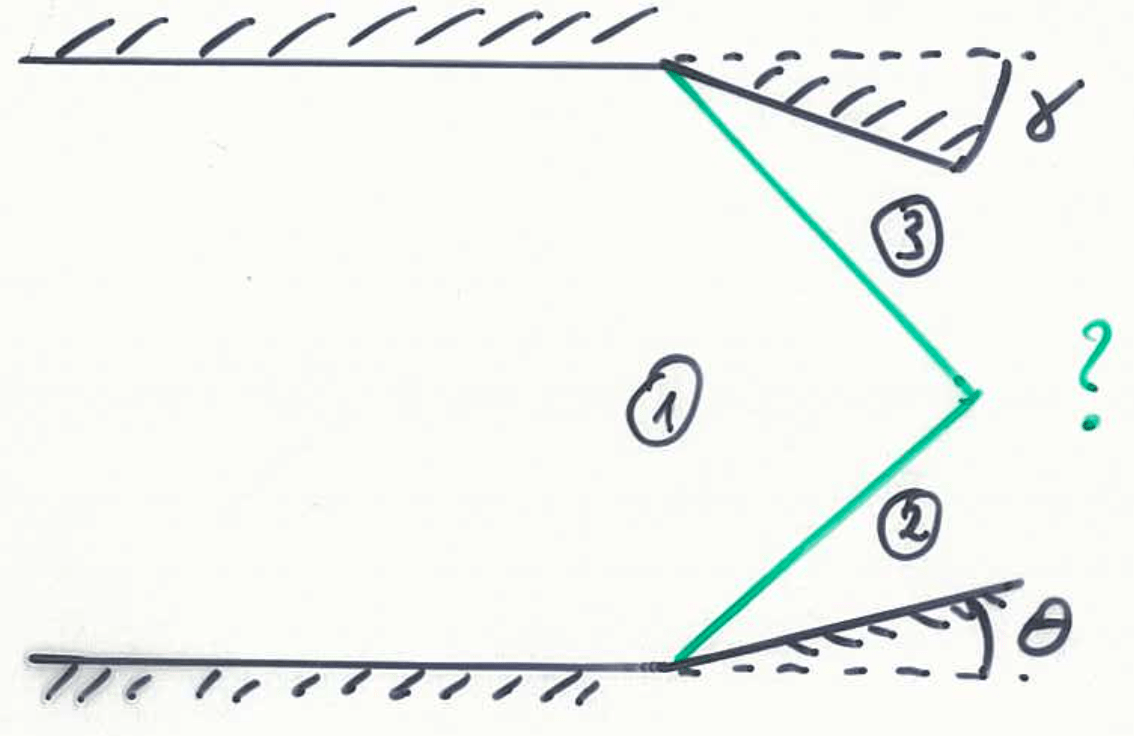
\includegraphics[scale=0.3]{ch2/8}
	\captionof{figure}{}
	\end{wrapfigure} 
	This figure represents a single-phase (where the input is an rms voltage $V_{ac}$) and a three-phase bridge (where the input is a phase-to-phase rms voltage $U_{ac}$). These bridges receive an AC voltage of frequency $f$ as an input. The output terminals furnish a DC voltage to a load. They are referred to as $P$ and $N$ and they are connected to the positive bus and the negative bus respectively. The instantaneous output voltage $v_{PN}(t)$ will be referred to as $v_{dc}(t)$. As both the positive and the negative alternations are employed these bridges are considered \textbf{full-wave rectifiers}. The input terminals are linked to the wire between two diodes. In the bridges the upper diodes ($D^i$) will work as maximum voltage selectors and the lower diodes ($D_i$) will work as minimum voltage selectors. This way, the instantaneous output voltage $v_{PN} \equiv v_{dc}$ is the maximum voltage amongst the input lines: 
	\begin{equation}
	\begin{aligned}
		single-phase &: v_{dc}(t) = \max (v_{ac}, -v_{ac}) = |v_{ac}|,\\
		three-phase &: v_{dc}(t) = \max (u_{ab}, -u_{ab}, u_{bc}, -u_{bc}, u_{ca}, -u_{ca})
	\end{aligned}
	\end{equation}
	
	\begin{wrapfigure}[10]{r}{4.2cm}
	\vspace{-5mm}
	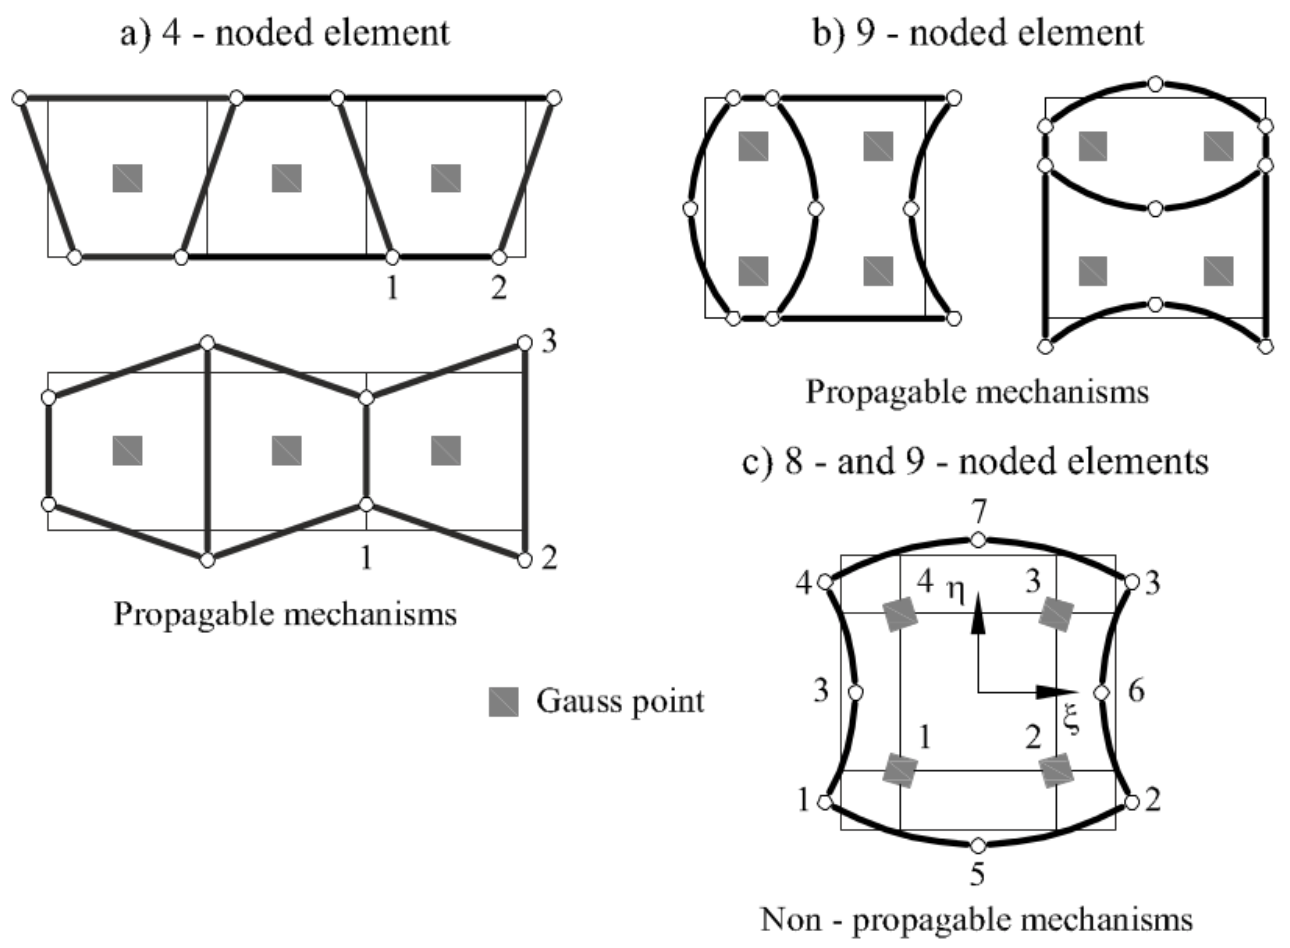
\includegraphics[scale=0.3]{ch2/9}
	\captionof{figure}{}
	\end{wrapfigure} 			
	This is easier to see graphically. We will only consider the upper envelope of the voltages as shown in the previous figure. We call it 2-pulse or 6-pulse rectification, which implies $2kf$ and $6kf$ harmonics in the spectres of the DC quantities.
	
	The output voltage of the three-phase bridge will be way less distorted ans it will fluctuate between $\sqrt{3/4}Û_{ac} = 0.866 Û_{ac}$ and $Û_{ac}$. Their average output voltages will be:
	\begin{equation}
		\begin{aligned}
		single-phase &: V_{dc} = \frac{1}{\pi}\int _{-\frac{\pi}{2}} ^ {\frac{\pi}{2}} \sqrt{2} V_{ac} \cos \omega t \, d\omega t = \frac{2\sqrt{2}}{\pi} V_{ac},\\
		three-phase &: V_{dc} = \frac{3}{\pi}\int _{-\frac{\pi}{6}} ^ {\frac{\pi}{6}} \sqrt{2} U_{ac} \cos \omega t \, d\omega t = \frac{3\sqrt{2}}{\pi} U_{ac},
		\end{aligned}
		\label{eq:2.14}
	\end{equation}
	The hypothesis needed to reach those values and conclusions were: 
	\begin{itemize}
		\item[•] The AC voltage source is ideal, $L_{ac} = 0$ (in practice $L_{ac}\neq 0$). 
		\item[•] Continuous conduction. In fact, we might have intervals during which any of the diodes conducts, when that happens $v_{dc}$ will only depend on the load. 
		\item[•] Ideal diodes (ideal characteristic). 
	\end{itemize}
	
\section{Bridges - operation with an inductive load (continuous conduction)}
	\subsection{Single-phase bridge and infinitely inductive load}
		\begin{wrapfigure}[4]{l}{4.5cm}
		\vspace{-5mm}
		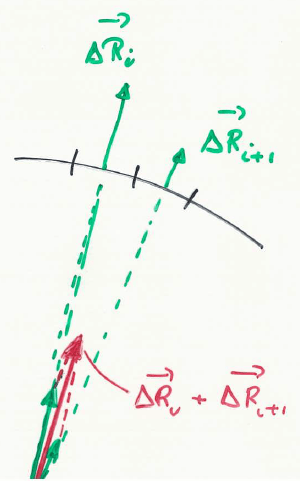
\includegraphics[scale=0.25]{ch2/10}
		\captionof{figure}{}
		\end{wrapfigure} 
		First, we consider an ideal AC load $L_{ac} = 0$ and a DC RLE load with $L_{dc}\rightarrow \infty$. During positive alternations of the input voltage $v_{ac}^0$, diodes $D^a$ and $D_b$ are conducting and during negative alternations diodes $D^b$ and $D_a$ will conduct. The smooth DC output current $i_{dc}$ implies a square-wave input current. The fact that $L_{ac} = 0$ allows the discontinuity of the current during commutations. The amplitude of the fundamental input current is $I_{ac,1} = \frac{2\sqrt{2}}{\pi} I_{dc}$. It is in phase with $v_{ac}^0$ and, consequently, $DPF = \cos \varphi _1 \approx 1$. That is the case of almost every diode rectifier. However, the $PF<1$ because of the distortion of the square-wave current. We can check the power balance with the equation \eqref{eq:2.14} : 
		\begin{equation}
			V_{ac}^0I_{ac,1} \cos \varphi _1 = V_{dc} I_{dc}.
		\end{equation}
		When $L_{dc} \neq \infty$, the current is not constant and it fluctuates with $I_{dc,min} \geq 0$. When $E_{dc}<V_{dc}$, the current will be continuous as long as $L_{dc}$ remains big enough. In this case, we have discontinuous conduction and \eqref{eq:2.14} is still valid. Taking into account the voltage drop in the diodes, we can increase the accuracy of this equation: 
		\begin{equation}
			V_{dc} = 0.9003 V_{ac}^0 - 2 V_{D,on} - 2 R_{D,on} I_{dc}
		\end{equation}
		
	\subsection{Three-phase bridges and infinitely inductive load}
		\begin{wrapfigure}[13]{l}{5.6cm}
		\vspace{-5mm}
		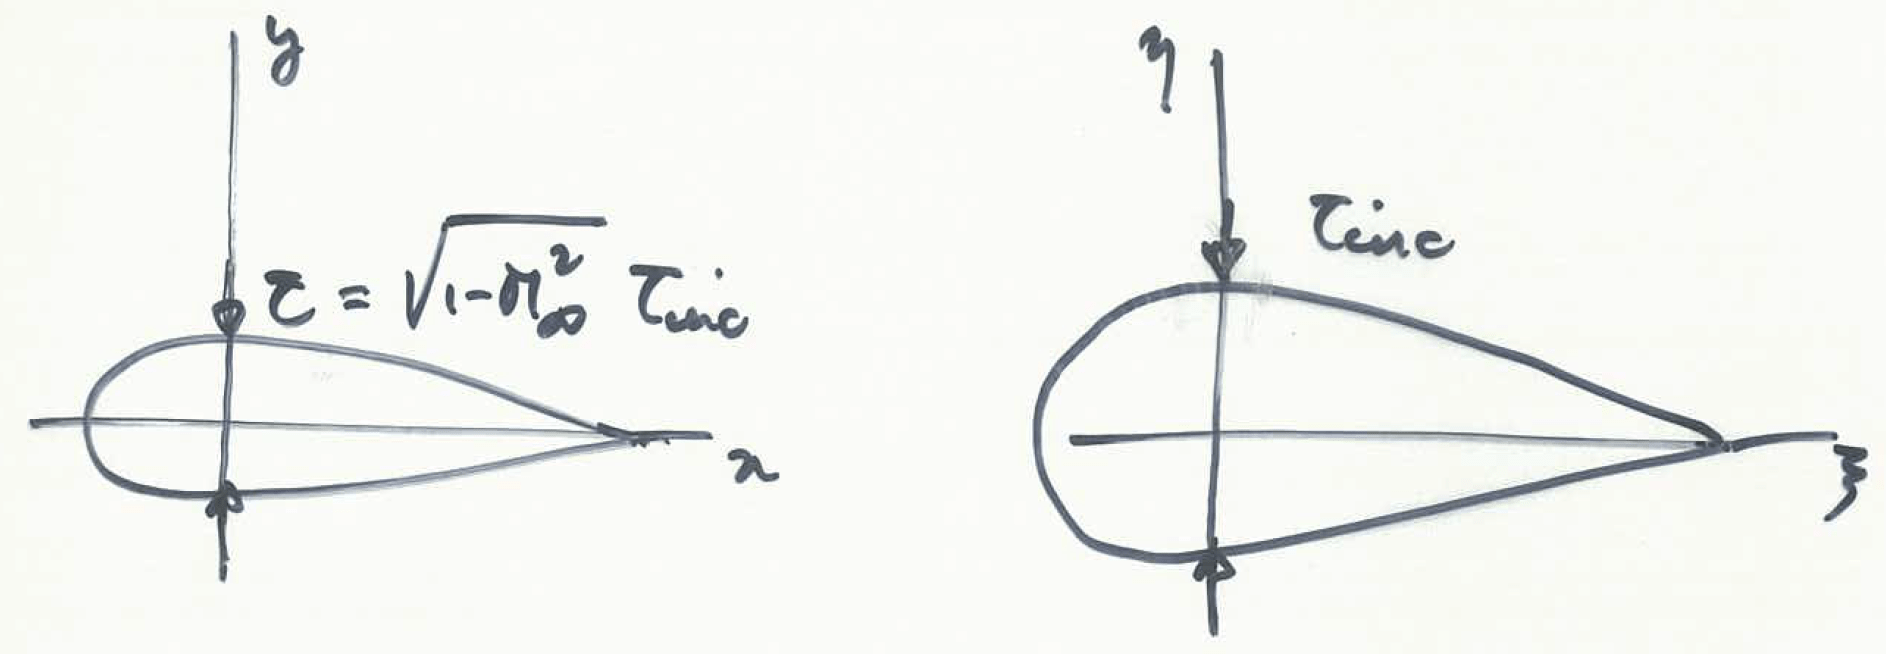
\includegraphics[scale=0.3]{ch2/11}
		\captionof{figure}{}
		\end{wrapfigure} 
		They operate following the same principle as the single-phase bridge. However, here each phase conducts during 2 times 120$^\circ$.\\
		The ideal voltage source is represented by its star connected equivalent circuit. We will consider $L_{dc} = \infty$ and the 3 phases will contribute symmetrically to the constant DC current. During a fundamental period, each phase will conduct for 2 times 120$^\circ$  and will block the current during 2 times 60$^\circ$. The 3 currents constitute a three-phase square wave. Once again, the fundamentals of the currents are in-phase with their respective voltages and $\varphi _1 = 0 \Rightarrow \cos \varphi _1 = 1$. The rms value of the fundamental component of the current is $I_{ac,1} = \frac{\sqrt{6}}{\pi}I_{dc}$. This way the power balance is:

		\begin{equation}
			\sqrt{2}V_{ac}I_{ac,1} \cos \varphi _1= V_{dc}I_{dc}. 
		\end{equation}
		
		In the \textbf{continuous} case, \eqref{eq:2.14} remains valid as long as we add the losses inside the 2 conducting diodes. 
		
	\subsection{Single-phase bridges, commutation between diodes}
	    
	    In a system we might have, besides the inner inductance of the source, a smoothing inductance or an LC filter after the diodes. When that happens the commutation cannot be immediate anymore. \\
		
	\begin{wrapfigure}[8]{r}{5cm}
		\vspace{-5mm}
		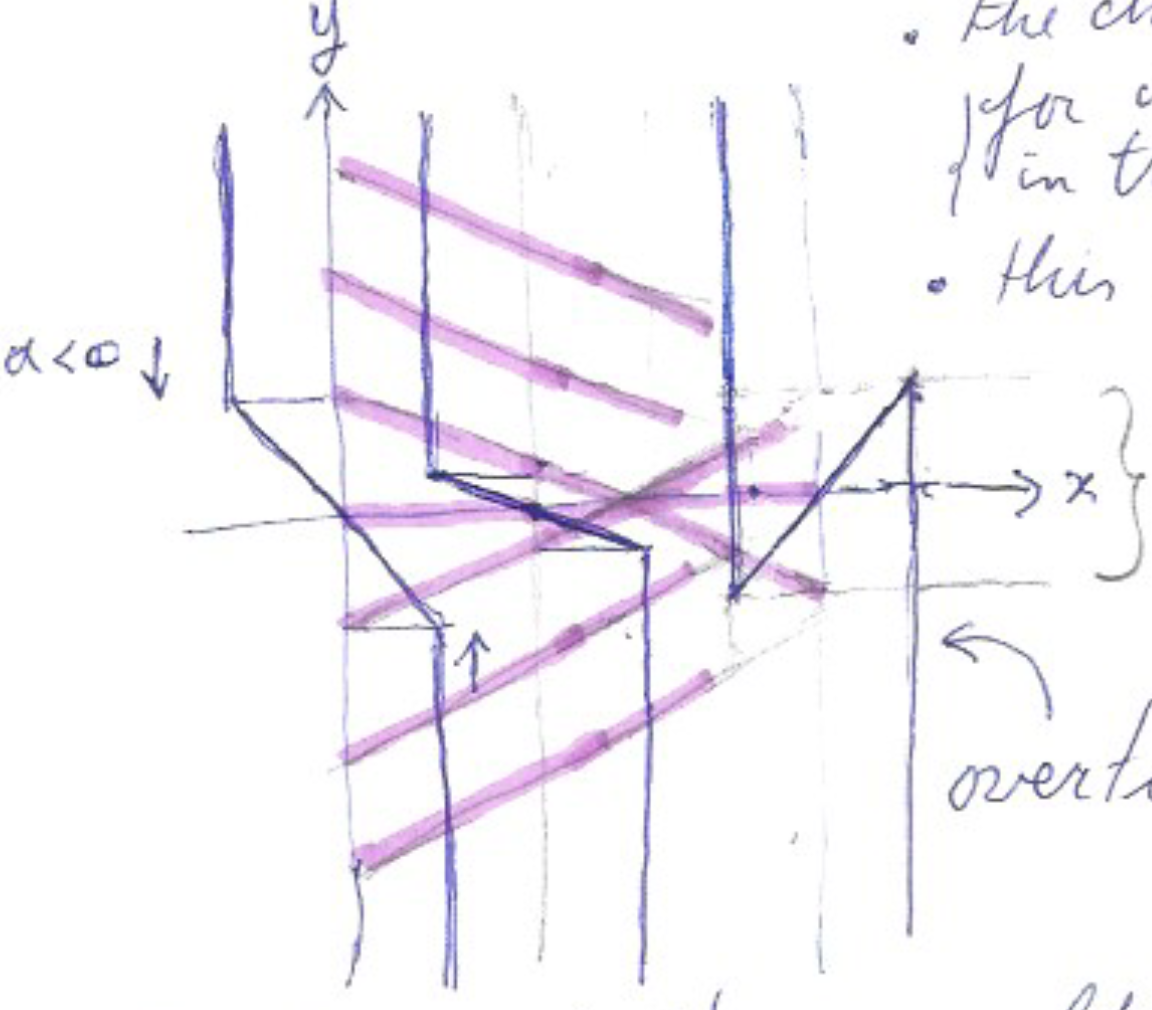
\includegraphics[scale=0.3]{ch2/12}
		\captionof{figure}{}
		\end{wrapfigure} 
		First we will study a circuit with an inductance before the rectifier $L_{ac} \neq 0$. The figure represents the commutation intervals $T_{com}$. We can demonstrate that with an infinitely inductive load the output voltage will be the average of those appearing during the commutation, thus nil. So the commutation will take: 
		\begin{equation}
			\omega T_{com} = \arccos \left( 1-\frac{2\omega L_{ac}}{\sqrt{2}V_{ac}^0} I_{dc}\right). 
		\end{equation}
		
		We can now calculate the drop of the average DC voltage: 
		\begin{equation}
			\Delta V_{dc} = \frac{2\omega L_{ac}}{\pi}I_{dc}. 
		\end{equation}
		
		\begin{wrapfigure}[5]{l}{4cm}
		\vspace{-5mm}
		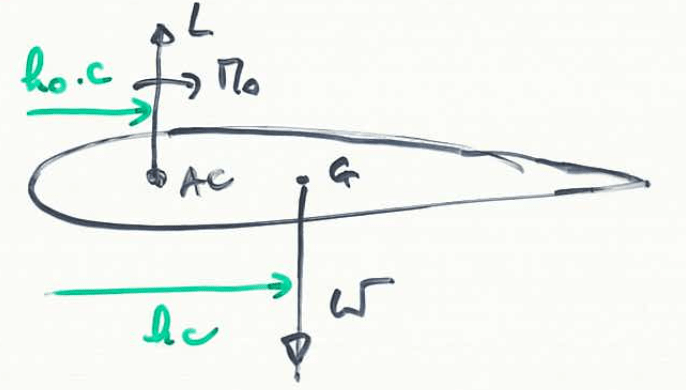
\includegraphics[scale=0.3]{ch2/13}
		\captionof{figure}{}
		\end{wrapfigure} 
		We can therefore express the average voltage with the voltage drops in the diodes and $\Delta V_{dc}$ then group together the DC voltage source with its inner resistance (Thevenin) : 
		\begin{equation}
			V_{dc} = \underbrace{0.9003 V_{ac}^0 - 2V_{D,on}}_{V_{dc}^0} - \underbrace{\left( 2 R_{D,on} + \frac{2\omega L_{ac}}{\pi} \right)}_{R_{i,dc}} I_{dc}
		\end{equation}
		This characterization of average values is only valid when conduction is continuous. It will become discontinuous when the current goes over a certain limit value called $I_{dc,lim}$. Because of the overlapping, the fundamental component of the current has a lag with respect to the voltage $v_{ac}^0$ with $\varphi _1 >0$ and $DF = \cos \varphi _1 < 1$. \\
		
		With a three-phase system, the obtained equations are: 
		\begin{equation}
			\omega T_{com} = \arccos \left( 1-\frac{2\omega L_{ac}}{\sqrt{2}U_{ac}^0} I_{dc}\right) \qquad \Delta V_{com} = \frac{3\omega L_{ac}}{\pi} I_{dc}.
		\end{equation}
		
\section{Diode bridges - operation with smoothing of the DC voltage (by a capacitor)}
    We will connect the capacity $C$ in parallel with the load in order to smooth the voltage. The distortion of $v_{dc}(t)$ will become smaller as we put bigger capacities. If the capacity is infinitely big the voltage will be perfectly smooth $V_{dc}$, but there are disadvantages to this solution: the energy and time needed to charge the capacity will also be infinite. For the moment, the load considered will only consist of a resistance $R_{dc}$. The voltage $v_{dc}(t) = v_C(t)$ will be linked to the current by the equation:
	\begin{equation}
		C\frac{dv}{dt} = i_C = i_{dc} - i_{dc,R}
	\end{equation}
	where $i_{dc}$ and $i_{dc,R} > 0$. At steady state, the rms value of the current flowing through the capacity $I_C = 0$. The DC current becomes $I_{dc} = I_{dc,R}$ and as Joules' law implies, it will be higher for smaller resistances. When there is no load, the open circuit will work as an infinite resistance $R_{dc}=\infty$ and thus there will be no conduction.
	
	\subsection{Single phase diode bridges with smoothing of the output voltage}
		\begin{wrapfigure}[7]{r}{7.5cm}
		\vspace{-5mm}
		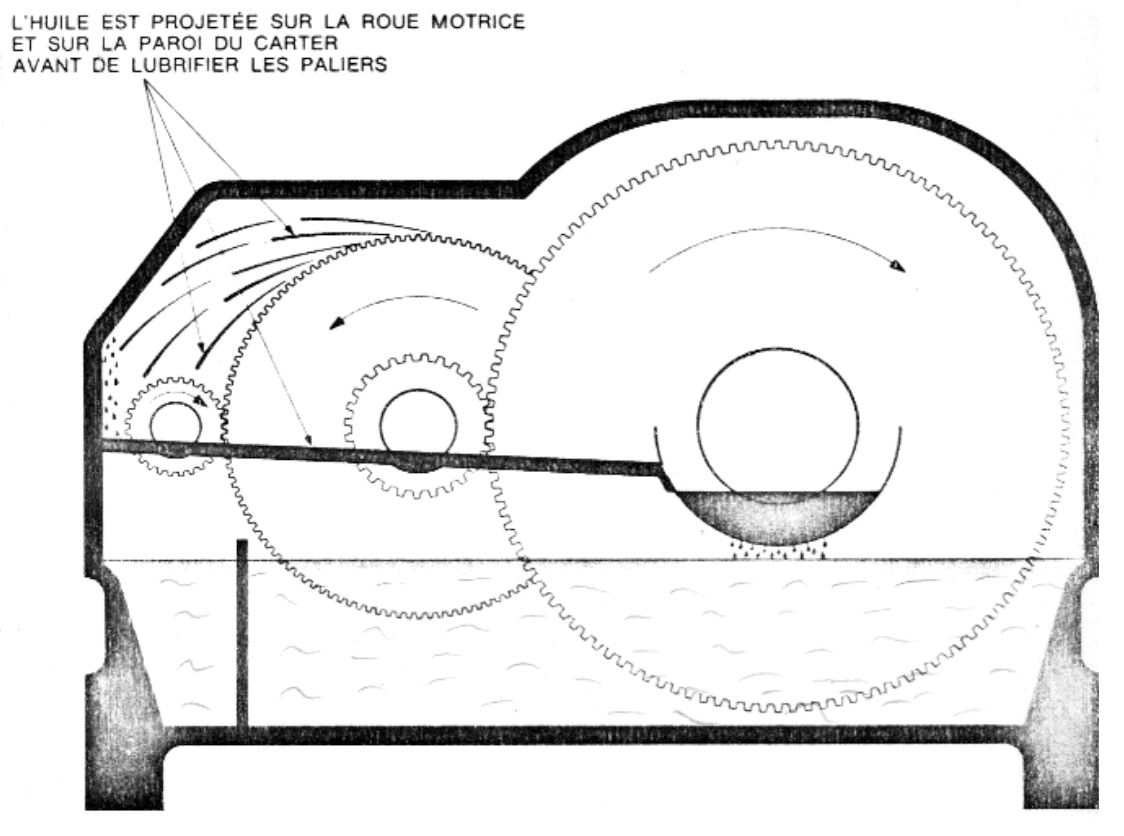
\includegraphics[scale=0.27]{ch2/14}
		\captionof{figure}{}
		\end{wrapfigure} 
		This circuit has three inductances, one corresponds to the inner impedance of the source $L_{ac,1}$, another one to the smoothing inductor at the input $L_{ac,2}$ and the last one to a second smoothing self $L_{dc}$. The inductors considered here are perfect, that is to say without inner resistance. Other loads can be connected to the source via the PCC, where the voltage is:
		
		\begin{equation}
			v_{ac}(t) = v_{ac}^0(t) - L_{ac,1}\frac{di_{ac}}{dt}.
		\end{equation}
		
		If we consider that $v_{ac}^0$ is perfectly sinusoidal (the only component is the fundamental harmonic), the only distortion is generated by the current $i_{ac}$. If we write the harmonic components of the voltage $v_{ac}^0(t)$ as a function of the rms values of harmonics of order $k>1$ of the current $i_{ac}(t)$:
		
		\begin{equation}
			v_{ac,k}(t) = -L_{ac,1}\frac{di_{ac,k}}{dt} \qquad \Rightarrow  V_{ac,k} = k\omega L_{ac,1} I_{ac,k}.
		\end{equation}
	    It is easy to see the interest of limiting the distortion of the current if we want to limit the distortion of the voltage. Thanks to the capacitor the output voltage will be barely distorted. We can model that RC load as an ideal DC voltage source whose value $V_{dc}=cst$ will be function of $R$. 
		
		\subsubsection{Discontinuous conduction}
			\begin{wrapfigure}[9]{l}{6cm}
			\vspace{-5mm}
			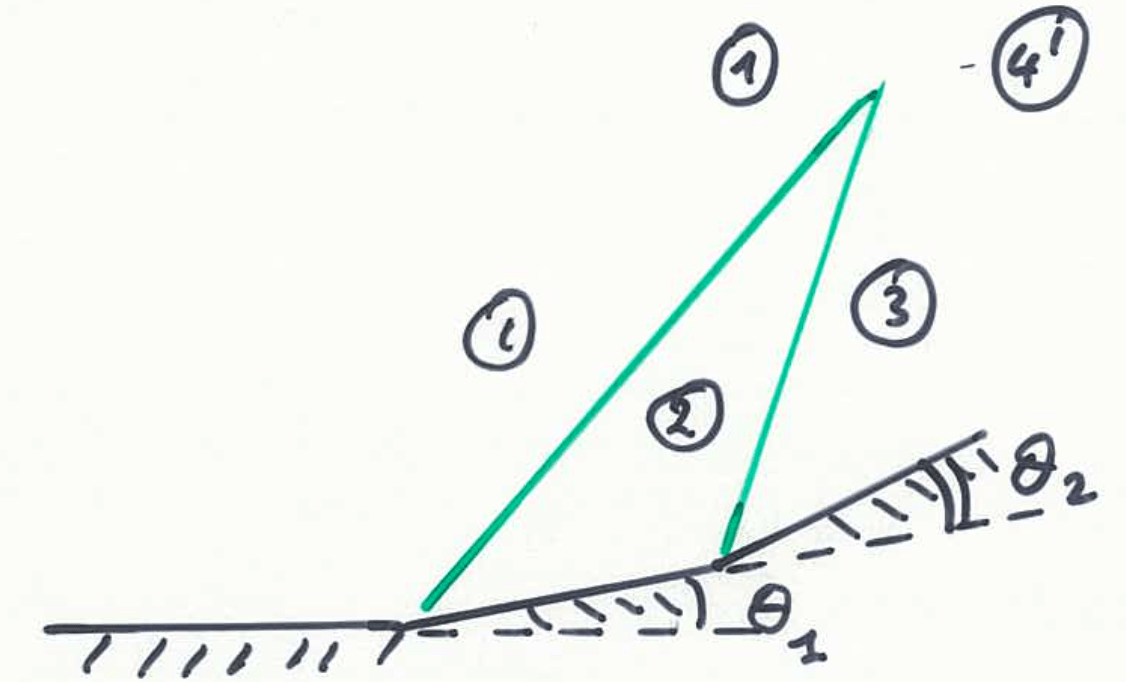
\includegraphics[scale=0.3]{ch2/15}
			\captionof{figure}{}
			\end{wrapfigure} 
			In this figure we can see the distortion of the output voltage. As there are intervals $T_{nc}$ during which $i_{ac} = 0$, conduction is discontinuous. These intervals are delimited by current impulsions that last $T_{c}$, with:
			\begin{equation}
				T_{nc} + T_c = \frac{T}{2}.
			\end{equation}
			
		    Conduction takes place by diode couple, without overlapping (4 diodes conducting simultaneously). The rectified current $i_{dc} = |i_{ac}|$ possesses 2 positive impulsions by fundamental period. The current $i_{ac} \neq 0$ only flows when $|v_{ac}^0(t)| \geq v_{dc}(t)$. Thanks to the total inductance $L_{ac} + L_{dc}$, the current $i_{ac}$ grows until it reaches its maximum when $|v_{ac}^0| = v_{dc}$. Conduction will last until the energy stored in the inductances runs out. During these conduction intervals $T_c$, the differential equations of the rise and the descent of $i_{dc}$ is:
			\begin{equation}
				(L_{ac}+L_{dc})\frac{d_{i_{dc}}}{dt} = |v_{ac}(t)|-v_{dc}(t).
			\end{equation}
			
			\textbf{Output voltage} \qquad In a real case, where $C$ is finite, $v_{dc}(t)$ has \textit{sawtooth} shape. The fluctuation will be lesser for higher capacities. During $T_{nc}$ (when $i_{dc} =i_{ac} =0$), the load and the capacitor are not fed by the source. Instead, the capacitor will use its stored energy to feed the load. If the time constant of the circuit $\tau = R_{dc}C$ is big with respect to $T/2$, the falling edges of the fluctuation are almost straight lines with a gradient $-V_{dc}/\tau$ : 
			\begin{equation}
				C\frac{v_{dc}(t)}{dt} = -i_{dc,R}(t) = \frac{v_{dc}(t)}{R} \qquad \Rightarrow \qquad \frac{dv_{dc}}{dt} \approx - \frac{V_{dc}}{R_{dc}C} \qquad (i_{dc} = 0).
			\end{equation}
			
			During a conduction interval $T_c$, $v_{dc} = v_c$ reaches a maximum value when $i_{dc} = i_{dc,R}$ as depicted in (Eq.:2.22)\eqref{eq:2.22}. The minimum output voltage will appear at the beginning of $T_c$ and the maximum at the end. The peak-to-peak ripple $v_{dc}(t)$ will be approximated as follows:
			\begin{equation}
				\Delta V_{dc,pp} \approx \frac{T_{nc}}{R_{dc}C}V_{dc},
			\end{equation}
			Its upper limit is obtained when $T_{nc} = T/2$.
			\\
			
			\textbf{Output current} \qquad As $v_{dc}$ is little distorted, the current $i_{dc} = v_{dc}/R_{dc}$ will be little distorted too. The current in the capacitor $i_c = i_{dc}-i_{dc,R}$ is the difference between $i_{dc}$ in thin impulsions $\pm$ and $i_{dc,R}$ is quasi constant. Remember: $i_c$ is an AC current with a nil average value at steady state. 
			\\
			
			\textbf{Dimensionless output voltage/current characteristics} \qquad We will focus on the global characteristic of the output, the average output voltage $V_{dc}$ versus the average output current $I_{dc}$ that is to say the load resistance $R_{dc}=V_{dc}/I_{dc}$, while considering a capacity big enough to neglect its effect on the characteristic. The remaining parameters are 

			\begin{wrapfigure}[8]{r}{6cm}
			\vspace{-5mm}
			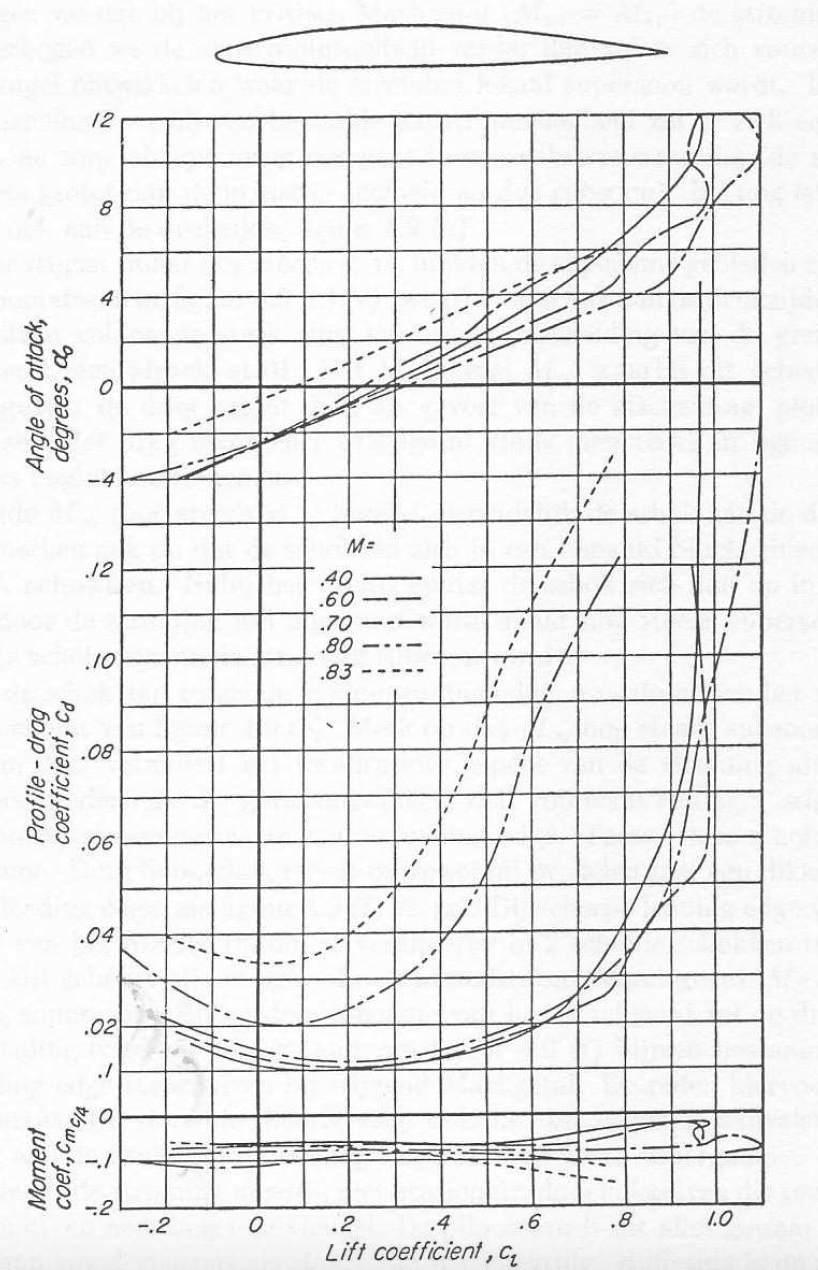
\includegraphics[scale=0.3]{ch2/16}
			\captionof{figure}{}
			\end{wrapfigure} 
			thus $V_{ac}^0, \omega$ and $L_{tot}$ (for the discontinuous case). We will render $V_{dc}$ and $I_{dc}$ dimensionless by dividing them by $V_{ref} = V_{ac}^0$ and $I_{ref} = V_{ac}^0/(\omega L_{tot})$. We can now represent the characteristic of the output with a single curve as in the figure. This curve won't change if we modify the values $V_{ac}^0, \omega$ and $L_{tot}$ as long as $C$ is big. We see that $V_{dc}$ grows closer to 
			$\sqrt{2}V_{ac}^0$ as the load diminishes ($R_{dc}$ growing, $I_{dc}$ shrinking). When we lack a load ($R_{dc} = \infty$, $I_{dc} = 0$), the capacitor remains charged at a voltage of at least $\sqrt{2}V_{ac}^0$ and current doesn't flow in the diode bridge. \\
			When the load increases ($R_{dc}$ shrinks), we go down the curve, $V_{dc}$ drops and $I_{dc}$ increases. That happens at the same time as the commutation intervals $T_c$ grow longer. Lastly we get to the limit betwee continuous and discontinuous conductino, where $T_c = T/2$ and the current impulsions merge. Trough numeric simulation we observe this limit at $I_{dc} \approx 0.3 V_{ac}^0/(\omega L_{tot})$, which corresponds to the point {0.3, 0.9} of the curve. The THD of $i_{ac}(t)$ growss bigger with minor loads. On the other hand, the lag of the fundamental component of $i_{ac}(t)$ with respect to $v_{ac}(t)$ is low, which gives a $DPF = \cos \varphi _1 \approx 1$. 
			
		\subsubsection{Discontinuous conduction}
			\begin{wrapfigure}[8]{l}{6cm}
			\vspace{-5mm}
			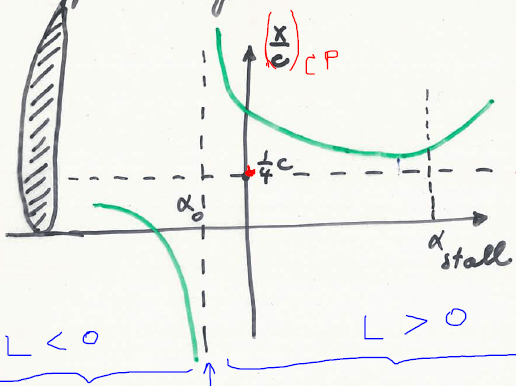
\includegraphics[scale=0.3]{ch2/17}
			\captionof{figure}{}
			\end{wrapfigure} 
			
			In this case, when $I_{dc}/I_{ref}>0.3$ the carried study becomes pertinent once again. The voltage $v_{dc}$ mainly constant thanks to the capacitor corresponds to an $E_{dc}$ of the load. $L_{dc}$ corresponds to the inner inductance of the load and it has little effect on the voltage. However, $L_{ac}$ is the cause of the encroachment that nullifies the output voltage. Through 3 simulations with different values of $L_{ac}$ and $L_{dc}$ while keeping the same $L_{tot}$, a variable $R_{dc}$ for each arrangement and a big constant capacity, we get these three curves. When $0<I_{dc}/I_{ref}<0.3$ conduction is continuous and the curves follow the same pattern. This shows that $L_{tot}$ is the inductance that will impose the characteristic of the system and not a single inductance by herself. For greater dimensionless currents, the dimensionless voltage will decrease linearly with the current because of the encroachment caused by $L_{ac}$.
			
	\subsection{Three-phase diode bridges}
	
		\begin{center}
		\begin{minipage}{0.45\textwidth}
			\begin{flushleft}
			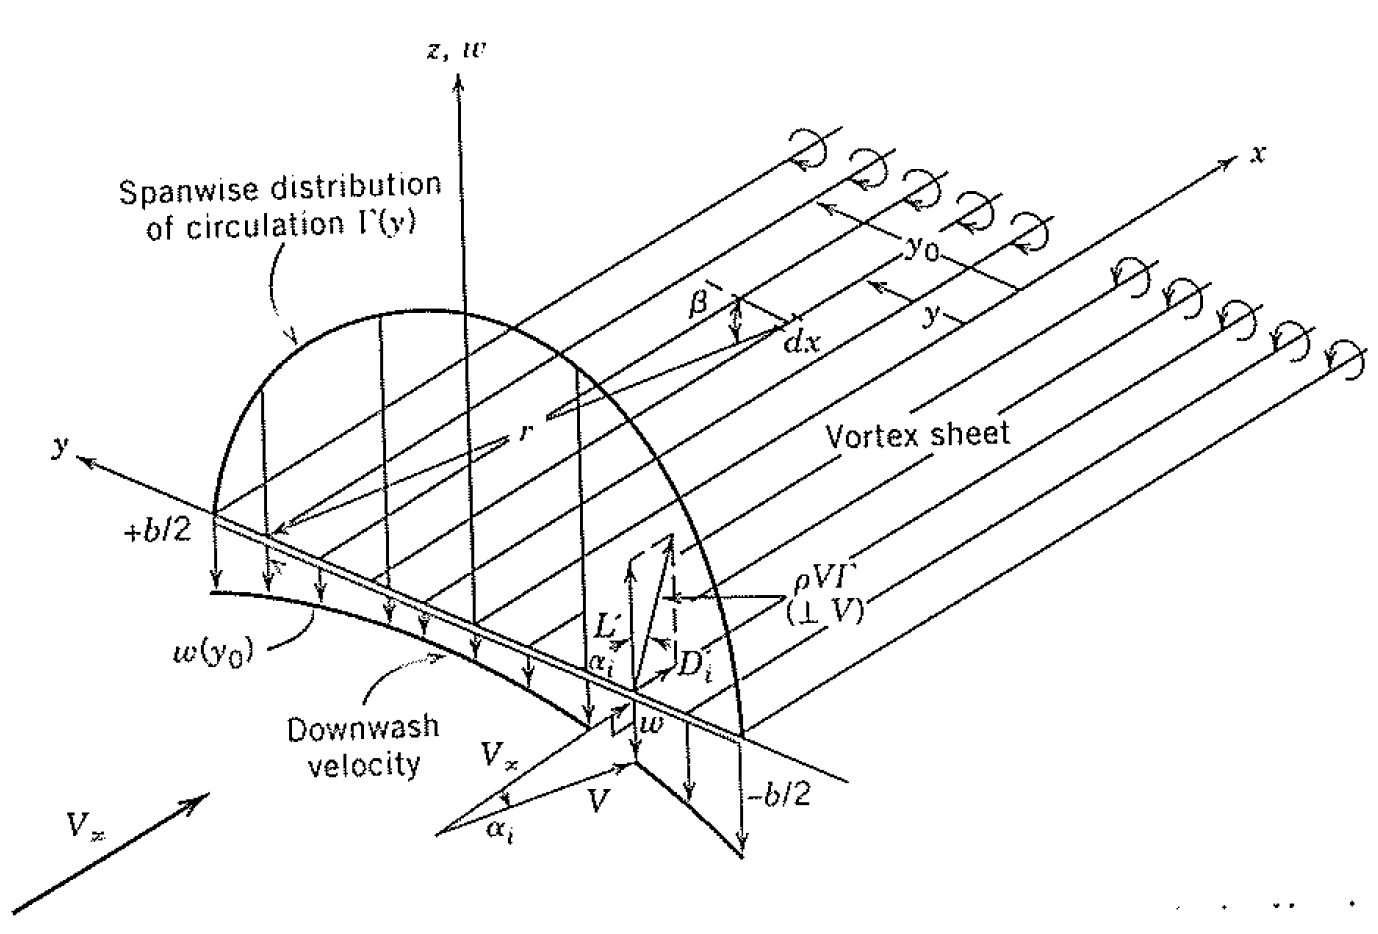
\includegraphics[scale=0.3]{ch2/18}
			\captionof{figure}{}
			\end{flushleft}
		\end{minipage}			
		\begin{minipage}{0.45\textwidth}
			\begin{flushright}
			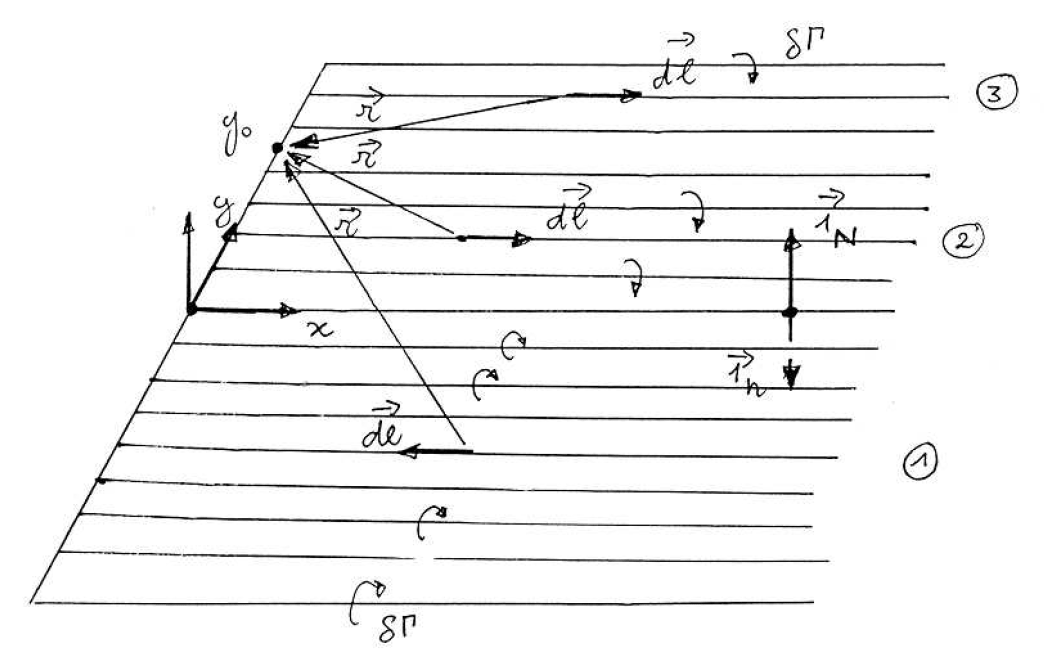
\includegraphics[scale=0.35]{ch2/19}
			\captionof{figure}{}
			\end{flushright}
		\end{minipage}			
		\end{center}
		
		This is the equivalent circuit of the three-phase system. In this figure each input line comprises the inductances $L_{ac,1}$ and $L_{ac,2}$ but there is a single $L_{dc}$ set after the rectifier. The classical shape of the AC current furnished by the source is also represented. When the current is continuous each phase current flows during 2 conduction intervals of 120$^\circ$. The depression between the conduction intervals of a single phase corresponds to the commutation between the two remaining phases as pointed in the figure.\\
		
		\textbf{Discontinuous conduction}\qquad When the load diminishes ($R_{dc}$ increases) and the conduction becomes discontinuous, the AC current contains 2 positive impulsions separated by an interval of non-conduction by fundamental period of the AC source. Each fundamental period also contains two negative impulsions showing the same phenomena as the positive ones. We have $i_{dc} = |i_{ac}|$ and during the conduction intervals the current flows through $L_{dc}$, two out of six diodes and two out of three input inductances $L_{ac}$. \\
		
		\begin{wrapfigure}[8]{l}{6cm}
		\vspace{-5mm}
		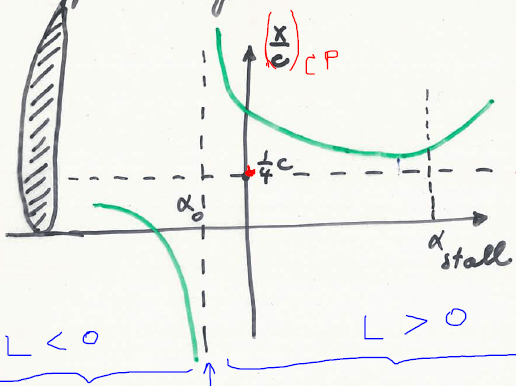
\includegraphics[scale=0.3]{ch2/17}
		\captionof{figure}{}
		\end{wrapfigure} 
		\textbf{Dimensionless output voltage/current characteristics}\qquad 		 We will choose as reference values $V_{ref} = U_{ac}^0$ and $I_{ref} = I_{ac}/(\omega L_{tot})$. This time it is appropriate to definite $L_{tot} = L_{dc}+ 2L_{ac}$. The simulation employed in the single-phase case is applied and the obtained curves appear in the graphic in the left. We remark the limit between discontinuous and continuous conduction at $I_{dc}/I_{ref} = 0.013$ and the ratio of 1.35 between $V_{dc}$ and $U_{ac}^0$ when conduction is discontinuous is easily observed. 
			